\chapter{Numerical Methods}

\section{Introduction}

In this section we want to introduce a part of the numerical methods, which were used in this thesis, for the performance of numerical computations.
To solve the in chapter () introduced equations of motion it is necessary to use spatial and temporal discretization schemes, to
compute the time evolution of fluid system from the initial state.
Different approaches like finite element and volume methods exist, here we will introduce the use of finite difference stencils for the
spatial and a third order runge kutta method for the discretization in time.
The choice of these methods in combination with the use of cartesian grids is in particular time saving when performing computations on the gpu, as we
will see in chapter ().

\section{Finite Differencing Schemes}

We start with a brief introduction of finite difference methods,
the interested reader is referred to [], for a more general overview, on which this section is primarly based on.
To begin with we will fall back on the one dimensional case, where we want to discretize the operators

\begin{align}
    \pdn[f]{x} \ , \ \pdn[^2f]{x^2}
\end{align}

for the function $f(x) blub$, such that the resulting error is as small as possible.
The idea behind finite differences is the same as to the original idea of the  derivative,
the approximation of the slope of a curve using neighboor points, except here we wont build the limit $dx>0$.
Suppose we want to calculate these derivatives on an intervall $I={xE}, L\in R$,
then we start by dividing $I$ into $N$ equidistant points $x_i; 0 seq i s 100$.

The distance between two neighboor ponits is giveb by $\Delta x = L/(N - 1)$.
Local to a single point $x_i$, we can now express $f$ using a taylor approximaton.

\begin{align}
    f(x) = f(x_i) + \left(\pdn[f]{x} \right)_i (x - x_i) + \left(\pdn[^2f]{x^2}\right)_i \frac{(x-x_i)^2}{2!}
\end{align}

Replacing $x$ with $x_{i+1}$ or $x_{i-1}$ and necgleting higher order terms, results in the following approximations for the first derivative.

\begin{align}
    \left(\pdn[f]{x}\right)_i &\approx \frac{f_{i+1} - f{i}}{\Delta x}\\
    \left(\pdn[f]{x}\right)_i &\approx \frac{f_{i} - f_{i-1}}{\Delta x}\\
    \left(\pdn[f]{x}\right)_i &\approx \frac{f_{i+1} - f_{i-1}}{2\Delta x}
\end{align}

\begin{figure}[!tpb]
  \centering
  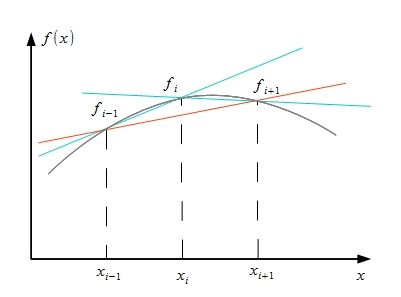
\includegraphics[width=0.6\textwidth]{gfx/numerik/fd_dummy.png}\label{fig:fd_schema}
  \caption{Approximation einer Funktion durch finite Differenznen}
\end{figure}

The first scheme is äquivalent to the definition of the first derivative, for $\Delta x \rightarrow 0$ and is also
denoted as forward difference, whereas the second scheme usually is referred to as backward difference.
The third approximation can be obtained by averaging over the first two approximations, and  is referred to as central difference.
The error resulting in the neglection of higher order terms in the taylor approximation, is denoted as the truncation error.
For the forward- and backward scheme this error is of first order, for the central scheme it is of second order.
All schemes are schematicaly shown in figure (), here the secord order central schemes results in the best approximationn.

\paragraph{Stability Analysis}\mbox{}\\

-beispiel erste abl dann zweit
-stabilität konstistenz - konvergenz etc
-verfahren höherer ordnung
-peclet zahl
-upwind schema


\section{Runge Kutta Verfahren}
Für die zeitliche Diskretierung wird ein Runge-Kutta Verfahren dritter Ordnung verwendet.
Ein Vorteil des Verfahrens dritter Ordnung ist die Stabilität gegenüber Oszillationen bei CFD-Problemen [QUOTE].
Allgemein wird bei der Herleitung

-warum ordnung 3
-runge kutta williamson etc
-stabilität
-fehler

\newpage

\section{Artificial Kompressibility}
bewegungsgleichungen
druckterm diskussion
exkurs laplace gleichung
beispiel rayleigh benard diskretisierung

